% ===================================================================
%  导言（Introduction） 原文：TASI10.tex 第 213--293 行（PDF p.2--5）
% ===================================================================
\section*{导言}

“月光”（moonshine）一词在数学中用来指模对象与有限群表示之间一种出人意料的联系。
过去五年间，对月光现象的研究进展迅速。这一联系虽然发生在两个数学结构之间，
人们却预期这种奇特联系的根源在物理，尤其是在弦论之中。

\vspace{2pt}
\begin{figure}[h!]
  \begin{center}
    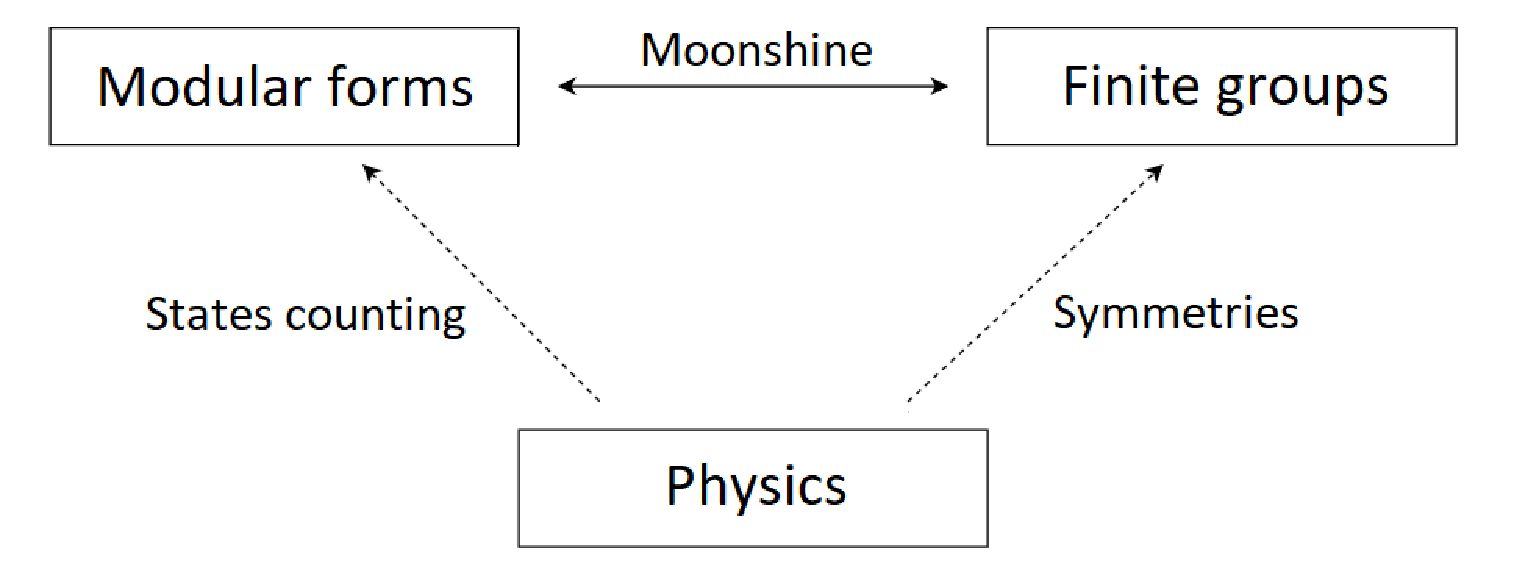
\includegraphics[width=0.66\linewidth]{figures/fig1_moonshine_diagram.pdf}
    \caption*{月光示意图。上方双向箭头表示模形式与有限群之间的“月光”联系；
    下方两条虚线分别表示“态计数”（states counting）与“对称性”（symmetries），
    意指两侧结构都通过物理（尤其是弦论）得到解释。原文此图无图注，位置见原文 p.2；
    本图注为译者所加，图中英文标注保持原样。}
  \end{center}
\end{figure}
\vspace{-8pt}

% [Tutor Note: “moonshine”一词由 Conway 与 Norton 在 1979 年引入，本义是“空谈、异想天开”，
% 用在此处带自嘲意味：两个毫不相干的数学结构竟由同一组整数联系起来，起初像是无稽之谈。
% 中文“月光”是约定俗成的译法，不要译作“月光效应”。]

\subsection*{月光：是什么、如何产生、为何重要？}

{\bf \em 问：什么是月光？}
\\\noindent
模形式的结构与有限群表示的结构先验地毫无关系。“月光”一词指的就是二者之间一种出人意料的联系。
但这个简单的回答会引出更多问题。月光出现在哪里？哪些类型的模对象会在月光关系中出现？
哪些类型的有限群可以被（模拟）模形式表示？以何种方式表示？这类月光关系是否存在某种分类？
在这些问题得到令人满意的回答之前，月光关系的存在在很大程度上仍是一个神秘现象。

\vspace{10pt}

\noindent
{\bf \em 问：月光关系是如何产生的？}\\\noindent
在经典情形——魔群月光（monstrous moonshine，Conway 月光亦然）——中，
相关的群表示具有顶点算子代数（vertex operator algebra，VOA）的结构，
详见第 \ref{cha:weight0} 节。用物理语言说，这些月光情形可以视为被某些特殊的
二维共形场论（conformal field theory，CFT）“解释”了：这些场论以相应的有限群为对称群。

% [Tutor Note: 这里“具有 VOA 结构”是精确说法：魔群月光模（即 McKay–Thompson 级数所对应的
% 无限维分次模）本身就是 Griess 代数（魔群 VOA）的表示空间；VOA 是二维手征共形场论的代数骨架，
% 由态—场对应把谱空间与算子代数等同起来。不要把 VOA 直接等同于 CFT：VOA 只编码手征（全纯）部分，
% 完整的 CFT 还需要反手征部分与模不变的内积（配分函数）。]

人们自然非常希望：对于本影月光（umbral moonshine）及其他新近发现的月光关系背后的有限群模，
也能有类似的物理构造。在某些“较简单”的情形里这已经实现
（参见第 \ref{sec:umbral} 节）。然而，能够反映本影月光全部二十三个实例统一结构的、
本影月光模的统一构造，至今仍然缺失。同样，其他各种新月光情形背后的模也尚未构造出来。

% [Tutor Note: 本影月光共有 23 个实例，与 24 个 Niemeier 格一一对应（除去无根的 Leech 格）；
% 这 23 个 Niemeier 格的根格决定了“本影群”与相应的模拟模形式。因此“二十三个”不是随意数字，
% 而是 Niemeier 格分类的直接结果——这也是原文强调“统一结构”的原因：23 个实例本应由同一个构造给出。]

除了“这些有限群模究竟是什么”这一问题之外，还有一个更深的问题：
“这些月光模具有何种（代数）结构？”新月光情形所涉及的模对象的\emph{模拟}
（mock）模性质似乎暗示：为了容纳相应的月光模，必须偏离人们熟悉的、具有离散谱的幺正共形场论。
不过，广义本影月光的存在（参见第 \ref{sec:umbral} 节）又暗示：
这些新模中仍应保留某些与全纯轨道流形共形场论相似的特征。

% [Tutor Note: 模拟模形式 $h(\tau)$ 不满足严格的模变换，其“影子” $g(\tau)$ 是权 $2-k$ 的模形式；
% 完备化 $\hat h(\tau)=h(\tau)+\text{非全纯修正}$ 才模不变。若把月光模当作某个 CFT 的谱生成函数，
% 则非全纯修正项对应连续谱的贡献，而这与“离散谱 + 幺正”的通常 CFT 公理冲突——这正是原文
% “必须偏离幺正离散谱 CFT”一段的物理含义。此处是理解新月光与经典月光差别的关键，勿轻易略过。]

最后但同样重要的是，本影月光的第一个实例——通常称为 Mathieu 月光——
是在弦论中 K3 曲面的背景下发现的。后续研究建立了 K3 弦论与本影月光全部二十三个实例之间的
密切关系。这一与 K3 弦论的联系是第 \ref{chap:moonshineK3} 节的主题。

% [Tutor Note: Mathieu 月光源于 Eguchi–Ooguri–Tachikawa（2010）对 K3 椭圆亏格的观察：
% K3 的椭圆亏格可分解为 $N=4$ 超共形特征标之和，其系数 $90,462,1540,\dots$ 恰为
% Mathieu 群 $M_{24}$ 的不可约表示维数（或分次维数）。这是“月光”在物理中首次被发现的实例，
% 也是后续本影月光猜想的出发点。]

总而言之，经典魔群月光的起源可以理解为：存在某种特殊的物理理论——
更准确地说，是某些二维手征 CFT 及相应的弦论嵌入。见第 \ref{cha:weight0} 节与
第 \ref{sec:physics_monstrous} 节。对新月光情形的起源的探索在很大程度上仍是一个富有挑战性的谜题。
不过，人们确实预期答案同样位于某些物理理论之中，而且多半来自弦论的框架。

\vspace{10pt}
\noindent
{\bf \em 问：为什么应当关心月光？}\\\noindent
以下是两位作者以及许多其他数学家、物理学家关心月光现象的一些理由。
首先，理论物理在很大程度上是研究对称性的，而月光在很大程度上是研究\emph{隐藏}对称性的，
这些对称性（据猜想）出现在物理情境之中。因此物理学家有充分理由关心月光领域的进展。
更一般地说，这一问题广泛的跨学科性质及其与数学和理论物理不同领域的联系表明，
理解这一数学范式很可能推动这些领域的新进展——经典魔群月光的情形显然正是如此。
下面我们结合近期进展，举出若干此类联系：

\begin{itemize}
\item  Mathieu 月光与本影月光的发现发端于 K3 弦论的背景，而 K3 紧化可以说是弦论中最重要的
       紧化范例之一。本影月光的发展一直为自守形式与 K3 几何的研究带来新结果，在弦论语境中尤其如此。
       我们预期它今后还会揭示 BPS 态的结构、非微扰黑洞量子态以及弦景观其他有趣侧面的信息。
       参见第 \ref{subsec:Mathieu}、\ref{sec:umbral} 节与第 \ref{chap:moonshineK3} 节。

\item  各种新月光实例的发现（参见第 \ref{ch:moonshineweight32} 节）涉及多种类型的有限群，
       其中包括一个无限族；这对理论物理提出了一个迷人的挑战：如何容纳相应的群表示。
       这一（提法完全明确的）谜题的解决，很可能指向物理中的新结构。

\item  某些新月光实例与算术几何之间的联系很有趣，并且可能成为通向数论新视角的一条富有成果的路径。
       参见第 \ref{ch:moonshineweight32} 节。
\end{itemize}

此外，模对象与有限群这两个截然不同的结构为何联系得如此之深，既令人着迷又令人困惑。
真正理解这些联系的本质，有可能深刻改变数学家看待这些对象的方式。

% [Tutor Note: 原文末尾“change the way mathematicians think about these objects”语气很重。
% 就历史看，魔群月光确实改写了人们对“有限群—自守形式”关系的认识（Borcherds 1992 年用
% 顶点代数与广义 Kac–Moody 代数证明魔群月光猜想，获 1998 年 Fields 奖），可作为理解本段分量的注脚。]

\subsection*{关于本讲义}

本讲义是为 2017 年 TASI 暑期学校中第二作者所作月光系列讲座而写的。

\subsection*{致谢}

第二作者感谢 TASI 2017 暑期学校的组织者给她在这个美好学校讲课的机会。
我们感谢 Sarah Harrison、Justin Kaidi、Natalie Paquette 与 Roberto Volpato
对早期草稿的评论。最后，第二作者感谢 Sarah Harrison、Jeff Harvey、Shamit Kachru、
Natalie Paquette、Brandon Rayhaun、Roberto Volpato、Max Zimet，
尤其感谢 John Duncan，感谢他们在相关课题上令人愉快的合作，也感谢他们教给我这个有趣课题的许多知识！
